%=========================================================================%
%   "Epigenetic basis of endocycle regulation in Oikopleura dioica"
%
% Master thesis by André Figueiredo Rendeiro
% 2013/1014
%
% University of Aveiro thesis
% based on the template by Tomás Oliveira e Silva
%
%=========================================================================%

\documentclass[11pt,twoside,a4paper]{report}
%incluir 'final' nas opções em baixo para omitir "Documento Provisório"
\usepackage[DBIO,newLogo,final]{uaThesis}

% optional packages
\usepackage[english]{babel}
\usepackage{hyperref}
\usepackage{amsmath}
\usepackage{amssymb}
\usepackage{xspace}% used by \sigla
\usepackage{cite}
\usepackage[titletoc]{appendix}
\usepackage{emptypage}

% provide encoding packages depending on the compiler
\ifxetex
  \usepackage{fontspec}
\else
  \usepackage[T1]{fontenc}
  \usepackage[utf8]{inputenc}
  \usepackage{lmodern}
\fi
% to get external fonts (e.g. google webfonts)
% must use xelatex compiler!!!
% \setmainfont[Ligatures=TeX]{Junge.ttf}

% defs
\def\ThesisYear{2014}
\def\ThesisAuthor{André Figueiredo Rendeiro}
\def\ptThesisTitle{Bases epigenéticas da regulação de endociclos em Oikopleura dioica}
\def\enThesisTitle{Epigenetic basis of endocycle regulation in Oikopleura dioica}

% optional (comment to use default)s
%   depth of the table of contents
%     1 ... chapther and sections
%     2 ... chapters, sections, and subsections
%     3 ... chapters, sections, subsections, and subsubsections
\setcounter{tocdepth}{4}

% optional (comment to used default)
%   horizontal line to separate floats (figures and tables) from text
\def\topfigrule{\kern 7.8pt \hrule width\textwidth\kern -8.2pt\relax}
\def\dblfigrule{\kern 7.8pt \hrule width\textwidth\kern -8.2pt\relax}
\def\botfigrule{\kern -7.8pt \hrule width\textwidth\kern 8.2pt\relax}

% custom macros (could also be defined using \newcommand)
\def\I{\mathtt{i}}         % one possible way to represent $\sqrt{-1}$
\def\Exp#1{e^{2\pi\I #1}}  % argument inside braces, i.e., "{}"
\def\EXP#1.{e^{2\pi\I #1}} % argument finishes when a full stop is encountered, i.e., "."
\def\sigla{\LaTeX\xspace}  % use as "blabla \sigla blabla (no need to do "blabla \sigla\ blabla"

\def\AddVMargin#1{\setbox0=\hbox{#1}%
                  \dimen0=\ht0\advance\dimen0 by 2pt\ht0=\dimen0%
                  \dimen0=\dp0\advance\dimen0 by 2pt\dp0=\dimen0%
                  \box0}   % add extra vertical space above and below the argument (#1)
\def\Header#1#2{\setbox1=\hbox{#1}\setbox2=\hbox{#2}%
           \ifdim\wd1>\wd2\dimen0=\wd1\else\dimen0=\wd2\fi%
           \AddVMargin{\parbox{\dimen0}{\centering #1\\#2}}} % put #1 on top #2

\begin{document}

%=========================================================================%
% Cover page (use only one of the first two \TitlePage)
%=========================================================================%
\TitlePage
    \HEADER{%\BAR\
    }{\ThesisYear}
    
    \TITLE{\ThesisAuthor}
        {\ptThesisTitle}
    \vspace*{10mm}
    \TITLE{}{\enThesisTitle}
          %\HEADER{\BAR\FIG{\begin{minipage}{50mm} % no more than 120mm
          %``I'm King of the world.''
          % \begin{flushright}
          %  --- Jack Nicholson
          % \end{flushright}
          % \end{minipage}}}
          % {\ThesisYear}
\EndTitlePage

\cleardoublepage

%=========================================================================%
% Cover page
%=========================================================================%

\TitlePage
    \HEADER{}{\ThesisYear}
    \TITLE{\ThesisAuthor}
        {\ptThesisTitle}
    \vspace*{10mm}
    \TITLE{}{\enThesisTitle}
    \vspace*{15mm}
    
    \TEXT{}
       {Dissertação apresentada à Universidade de Aveiro para cumprimento dos requisitos necessários à obtenção do grau de Mestre em Biologia Molecular e Celular, realizada sob a orientação científica de Eric Thompson, Professor do Departamento de Biologia da Universidade de Bergen e de Manuel Santos, Professor Associado do Departamento de Biologia da Universidade de Aveiro.}
       
\EndTitlePage

\cleardoublepage

%=========================================================================%
% Title page
%=========================================================================%

\TitlePage
  \vspace*{55mm}
  \TEXT{\textbf{jury}}{}
       
  \TEXT{president}
       {\textbf{António MASADASDDSASD}\newline {\small Associated Professor at the Biology Department of the University of Aveiro }}
  \vspace*{5mm}
  
    \TEXT{}
       {\textbf{António MASADASDDSASD}\newline {\small Associated Professor at the Biology Department of the University of Aveiro }}
  \vspace*{5mm}
  
    \TEXT{}
       {\textbf{António MASADASDDSASD}\newline {\small
        Associated Professor at the Biology Department of the University of Aveiro }}
  \vspace*{5mm}
  
\EndTitlePage

\cleardoublepage

%=========================================================================%
% Dedications
%=========================================================================%

\TitlePage
  \vspace*{55mm}
    \TEXT{\textbf{acknowledgements}}
        {I thank Prof. Thompson for allowing me to work in his lab and for all help with my stay in Norway. Pavla, for unconditional support and guidance during this period, Gemma for irreplaceable computational help, and everyone in the lab for all the good laughs and help when needed.}
    \TEXT{}
        {I'd like to thank my family for all the support throughout these years, allowing me to follow my dreams.}
    \TEXT{}
		{I'd also like to acknowledge the free open source software community for its marvellous efforts in building an open world and Tomás Oliveira e Silva for the University of Aveiro \LaTeX thesis template.}
    \TEXT{}
        {This thesis was made using entirely free open source software.}


\EndTitlePage

\cleardoublepage

%=========================================================================%
% Portuguese abstract page
%=========================================================================%

\TitlePage
  \vspace*{55mm}
  \TEXT{\textbf{palavras-chave}}
        {epigenética, endociclos, Oikopleura dioica}
  \TEXT{\textbf{resumo}}
    	{Lorem ipsum dolor sit amet, consectetur adipisicing elit, sed do eiusmod tempor incididunt ut labore et dolore magna aliqua. Ut enim ad minim veniam, quis nostrud exercitation ullamco laboris nisi ut aliquip ex ea commodo consequat. Duis aute irure dolor in reprehenderit in voluptate velit esse cillum dolore eu fugiat nulla pariatur. Excepteur sint occaecat cupidatat non proident, sunt in culpa qui officia deserunt mollit anim id est laborum.}
\EndTitlePage

\cleardoublepage

%=========================================================================%
% English abstract page
%=========================================================================%

\TitlePage
    \vspace*{55mm}
    \TEXT{\textbf{palavras-chave}}
        {epigenetics, endocycles, Oikopleura dioica}
  \TEXT{\textbf{abstract}}
		{Lorem ipsum dolor sit amet, consectetur adipisicing elit, sed do eiusmod tempor incididunt ut labore et dolore magna aliqua. Ut enim ad minim veniam, quis nostrud exercitation ullamco laboris nisi ut aliquip ex ea commodo consequat. Duis aute irure dolor in reprehenderit in voluptate velit esse cillum dolore eu fugiat nulla pariatur. Excepteur sint occaecat cupidatat non proident, sunt in culpa qui officia deserunt mollit anim id est laborum.}
\EndTitlePage

\cleardoublepage

%=========================================================================%
% Tables of contents, of figures, ...
%=========================================================================%

\pagenumbering{roman}

\tableofcontents
\cleardoublepage

%\listoffigures
\listoffigures
\cleardoublepage

%\listoftables
\listoftables
\cleardoublepage

%=========================================================================%
% The chapters (usually written using the isolatin font encoding ...)
%=========================================================================%
\pagenumbering{arabic}
%=========================================================================%
\chapter{Introduction}
%=========================================================================%

	\section{Epigenetics and Gene Regulation}
	

		\subsection{Histone Variants}
		

		\subsection{lncRNAs}
		

		\subsection{Histone modifications}
		

	\section{\textit{Oikopleura dioica}, a cross-disciplinary model system}
		\textit{Oikopleura dioica} is a marine chordate organism belonging to the class Appendicularia, which is a member of the Tunicate subphylum along with the classes Thaliacea (salps) and Ascidiacea (sea squirts). Tunicates are the most closely extant group related to the vertebrates (see Figure ~\ref{fig:tree}). \textit{Oikopleura} shares some biological traits with most tunicates (\textit{e.g.} filter feeding), but unlike them has some peculiarities which make it a very interesting model for the study of many biological features. \textit{Oikopleura dioica} owes its name to the fact that it is the only dioeicious appendicularian known, being most other species hermaphrodites.
		
		\begin{figure}[here]
			\centering
			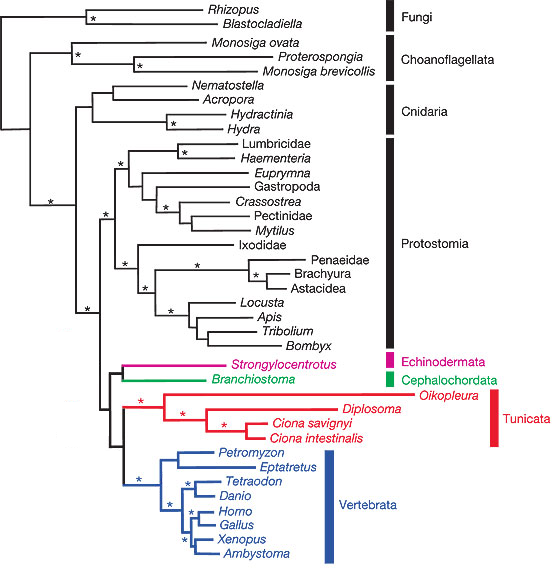
\includegraphics[width=0.5\textwidth]{tree.jpg}
			\caption{Phylogeny of the Deuterostome group with emphasis on the Tunicate subphylum}
			\label{fig:tree}
		\end{figure}
		
		\subsection{	\textit{Oikopleura}'s life cycle}
		\textit{Oikopleura} reproduces through external fertilization after the rupture of both female and male gonads or sperm release via the spermiduct \cite{}. The first cell division remarkably occurs only 35 min after fertilization and a XXXXXXX gastrulation takes place after two hours when at 20ºC. Four hours after fertilization the animal is ventrally bent with on its tail (Tailbud stage) and later hatches from the chorion to be a free-swimming larva. Figure \ref{fig:LifeCycle} represents the early development of \textit{Oikopleura}.
		
		Larval development takes place until fifteen hours after fertilization, where a metamorphosis known as Tailshift occurs and the tails changes orientation towards the ventral side of the animal. At this point, most cells stop mitotic division and start performing endocycling, a endoreduplicative cell division strategy which gives rise to multinucleated cells and increases body size by increasing the cell volume (discussed in detail in Section \ref{subsection:CellCycleVariants}). This strategy continues throughout most of the remaining juvenile life of \textit{Oikopleura} until the third day of development, where gametogenesis starts in the rapidly growing gonad. Most of \textit{Oikopleura}'s growth until the end of its life at day six is dedicated to gonad maturation, which at its peak reaches a total volume bigger than the somatic part of the whole organism. This is achieved again through the employment of endocycling in the gonad.
		
		\begin{figure}[here]
			\centering
			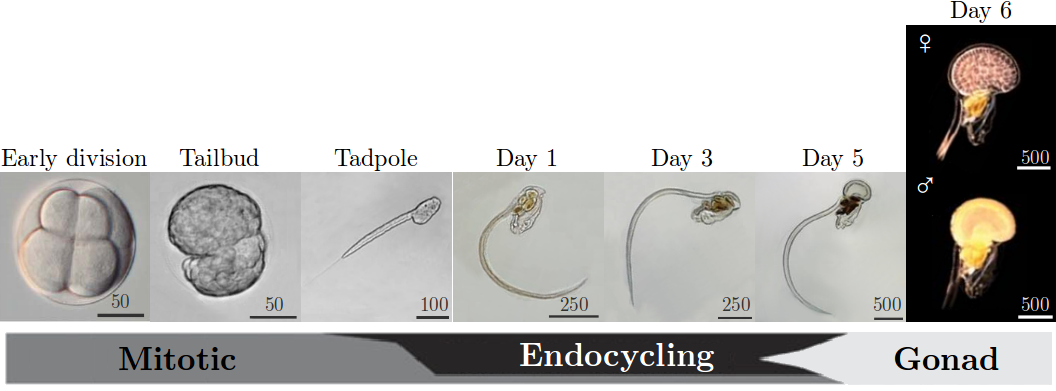
\includegraphics[width=0.5\textwidth]{lifeCycle.jpg}
			\caption{Diagram of \textit{Oikopleura dioica}'s development through its life cycle}
			\label{fig:LifeCycle}
		\end{figure}
		

		\subsection{The genome of \textit{Oikopleura dioica}}
		\textit{Oikopleura} reference genome sequence was made available in 2010 \cite{}, revealing a surprisingly plastic architecture and the species fast evolution.

		% compact
		In this planctonic animal, the chordate genome architecture seems to have been redesigned to obtain a minimal-sized genome: approximately 70 megabases. This is greatly due to the reduction of intron and intergenic space, although some gene loss also could also be detected. The dramatic reduction of intergenic space brings obvious constrains in terms of gene regulation, which is to some degree easily seen by the normal occurrence of genes in Operons (~28\% of the 18000 total), but makes the \textit{Oikopleura} genome one of the most compact of all known chordate genomes.
		Operons are significantly enriched for genes involved in house-keeping functions, while genes involved in developmental processes are significantly under-represented in Operons.
		Although a generalised change in cis regulatory modules seems a plausible hypothesis, cis regulation seems to take place. Highly Conserved Elements have been found through genomic alignments between Atlantic and Pacific \textit{Oikopleura dioica}.
		
		Nevertheless, several conserved genomic features can be found in the \textit{Oikopleura} genome.
		Long introns are more likely to be old than are short ones.
		Developmental genes show a double proportion of old introns compared to all annotated genes.
		

		\subsection{Cell cycle variants in \textit{Oikopleura dioica}}
		\label{subsection:CellCycleVariants}
		O. dioica displays an unique system of cell cycle regulation that is poorly understood, because previous research on cell cycle have focussed on a single nuclei within its own cytoplasm, while in this model we can study cell cycle regulation of multiple nuclei, both meiotic and endocycling, sharing a common cytoplasm, as seen in the coenocyst. Cell cycle in O. dioica is also unique in its way of development because most cells switch from rapid mitotic division to endoreduplication around the event of tail shift. O. dioica is also an important organism when viewed at the light of evolution, because it is the closest evolutionary relative to the vertebrates, and is therefore an important model organism in the field biology. In addition to presenting a unique environment for cell cycle studies and its evolutionary importance, it has many other abilities that make it an excellent model organism. O. dioica is successfully maintained in culture and have a short life cycle of 6 days at 15°C (Bouquet, 2009), and is therefore an excellent model organism for developmental studies. It is also transparent which makes it easy to observe internal organs when used for in situ experiments. Another advantage of using O. dioica as a model organism is the fact that the genome of O. dioica has been fully sequenced, which makes genetic studies easier by far.
		
			\subsubsection{Endocycling}
		
		\subsection{Histone variants in \textit{Oikopleura dioica}}
		\cite{Moosmann2011}

canonical core histones:
	replication dependent (RD) genes
	lack introns
	organized in gene clusters
	mRNAs possess a conserved stem-loop (SL) in the 3’UTR coupling gene expression to DNA replication

histone variants:
	are often transcribed from orphan genes
	contain introns
	lack the SL and their expression is not restricted to S-phase
	they are referred to as replacement or replication-independent (RI) variants.

H4 is highly constrained as it contacts with the other 3 core histones and its N-terminal tail residues are subject to extensive PTMs.
		

	\section{Endocycle regulation}
		\subsection{Advantages of endocycles}
		\subsection{Mammals}
		\subsubsection{Giant cell Placenta}
		\subsubsection{Liver}
		\subsection{Oikopleura}
		\subsubsection{Histone variants}

		\subsection{New insigts on endocycle control from epigenetics}
			\subsubsection{E2F family}
			\subsubsection{Dot1L}
			\subsubsection{DOT1L in cell reprogramming}

		\subsection{Project Goals}
		Identify the roles of the Oikopleura E2F TF family in endocycles
		Gain insights on the epigenetics basis for endocycle regulation mediated by H3K79me and it's methyltransferase Dot1L

\clearpage

%=========================================================================%
\chapter{Materials and Methods}
%=========================================================================%
	\section{Materials}
		\subsection{Antibodies}
			\begin{table}[!ht]
       		\caption{
            		\bf{Primary antibodies used for ChIP, immunofluorescence and western blot}
        }
        		\begin{center}
            		\begin{tabular}{|c|c|c|c|}
                		\hline
	                Antibody & Description & Supplier & Purpose\\
    		            \hline
        		        ab46540 & Rabbit Control IgG - ChIP Grade & Abcam & ChIP\\
            		    ab10543 & Anti-Histone H3 (phospho S28) [HTA28] & Abcam & ChIP\\
	                \hline
	            \end{tabular}
    		    \end{center}
		    \end{table}
		  
		\subsection{Chemicals and reagents}
			\begin{table}[!ht]
       		\caption{
            		\bf{Chemicals and reagents used in various protocols}
        }
        		\begin{center}
            		\begin{tabular}{|c|c|c|}
                		\hline
	                Chemical & Supplier & Purpose\\
    		            \hline
        		        X & X & X\\
	                \hline
	            \end{tabular}
    		    \end{center}
		    \end{table}
    
    		\subsection{Instruments and equipment}
			\begin{table}[!ht]
       		\caption{
            		\bf{Instruments and equipment used in various protocols}
        }
        		\begin{center}
            		\begin{tabular}{|c|c|c|}
                		\hline
	                Instrument/equipment & Supplier & Purpose\\
    		            \hline
					X & X & X\\
	                \hline
	            \end{tabular}
    		    \end{center}
		    \end{table}
		    
		\subsection{Buffers and solutions}
			\subsubsection{ChIP}
				\begin{table}[!ht]
       			\caption{
            			\bf{Lysis buffer}
            		}
	        		\begin{center}
    		        		\begin{tabular}{|c|c|}
        		        		\hline
	        		        Chemical & Concentration\\
    		        		    \hline
						X & X\\
		                \hline
		            \end{tabular}
    			    \end{center}
			    \end{table}
			    
			    \begin{table}[!ht]
       			\caption{
            			\bf{Lithium chloride buffer}
            		}
	        		\begin{center}
    		        		\begin{tabular}{|c|c|}
        		        		\hline
	        		        Chemical & Concentration\\
    		        		    \hline
						X & X\\
		                \hline
		            \end{tabular}
    			    \end{center}
			    \end{table}
			    
			    \subsubsection{Western blot}
				\begin{table}[!ht]
       			\caption{
            			\bf{Lysis buffer}
            		}
	        		\begin{center}
    		        		\begin{tabular}{|c|c|}
        		        		\hline
	        		        Chemical & Concentration\\
    		        		    \hline
						X & X\\
		                \hline
		            \end{tabular}
    			    \end{center}
			    \end{table}
		    		    
		    
	\section{Animal culture and collection}
		\subsection{Culture of \textit{O. dioica}}
		The culture of \textit{Oikopleura} was performed at the SARS centre appendiculatian facility as previously described \cite{Bouquet2009}. Cultured animals are native from the coastal area outside Bergen and are frequently collected and added to the permanent culture. Animals are permanently cultured at the facility in 6L seawater beakers, with permanent stirring and daily water renewal as well as feeding twice daily with algae according to the developmental stage (see table \ref{table:ODculture}). The use of a fixed volume for culture implies the progressive dilution of animals until the third day of life, where density remains at 150 animals per 6L beaker.
		
		\begin{table}[!ht]
       		\caption{
            		\bf{Feeding regime of \textit{Oikopleura} according to developmental stage}
        }
        		\begin{center}
            		\begin{tabular}{|c|c|c|c|c|c|}
                		\hline
	                \multicolumn{2}{c}{Developmental stage} & \multicolumn{4}{c}{Algae}\\
	                \hline
	                \multicolumn{2}{c}{} & Isochrysis sp. (cells/mL) & Chaetoceros calcitrans (cells/mL) & Rhinomonas reticulata (cells/mL) & Synecococcus sp. (mL) & crushed Rhinomonas reticulata (mL)\\
    		            \hline
        		        Day 1 & Morning & 2000 & 2000 & 0 & 5 & 5\\
        		        Day 1 & Evening & 1000 & 1000 & 0 & 3 & 5\\
	                \hline
	            \end{tabular*}
    		    \end{center}
        		\label{table:ODculture}
		    \end{table}
		
		\subsection{Collection of \textit{O. dioica}}
			\subsubsection{Tailbud stage}
			To collect \textit{Oikopleura} in the Tailbud developmental stage, a controlled \textit{in vitro} fertilization was performed. Day six mature male animals were collected to a Petri dish with seawater and allowed to spawn. When all male animals had spawned, sperm quality was visually inspected on a light microscope for motility. Day six mature females were individually collected to glass salliers with seawater and allowed to spawn at 18ºC. When spawned, 60µL of sperm solution was added to the sallier and after 3-4 hours tailbud animals collected to a eppendorf microtube.
			
			\subsubsection{Day two stage}
			Late day two \textit{Oikopleura} were individually collected with the aid of a 2 mL plastic pipette to a 1 L beaker with clean seawater (no algae) and stayed there 3 to 4 hours to be allowed to empty the gut of any remaining algae as well as build a new clean house.
			To achieve release of the houses, animals were individually collected again, this time using a mouth-pipette built from a 1 mL plastic pipette and poured into a glass recipient on ice with 0.125 mg/mL MS222 and allowed to sink to the bottom, where a third collection using a 200 µL micropipette took them to a 1.5 mL microtube.
			
			\subsubsection{Day six, immature stage}
			Immature day six animals with a visible gonad but naked-eye indistinguishable features were collected from culture into a 500 mL plastic beaker with clean seawater with the aid of a 25 mL plastic pipette and from there to a 1.5 mL microtube with a 2 mL plastic pipette. 
		
	
	\section{ChIP-seq}
		\subsection{ChIP}
			\subsubsection{Animal fixation}
			Tailbud and day two animals were briefly spin at 5000 g for 10 seconds to be collected at the bottom of the microtube, while day six immature voluntarily sank in seconds time. Seawater was exchanged for 0,5 mL PBS and 0,5 ml of either 1 or 2\% Formaldehyde in PBS was added to have a final fixative concentration of 0.5 or 1\% respectively, and let rotating for a variable amount of time as shown in Table \ref{table:ODfixation}, depending of the developmental stage. %Use good quality, methanol-free formaldehyde (see materials) and always opened fresh.
			
			Formaldehyde was quenched with Glycine solution to stop fixation and again let rotating for 5 min at 18ºC. 
			Again by either spinning at 5000 g for 30 seconds or allowing animals to freely sink, Formaldehyde was removed and animals washed with cold PBSplus three times on ice, after which all solution was removed and animal pellets frozen with liquid nitrogen and stored at -80ºC for future use.
    
    \begin{table}[!ht]
        \caption{
            \bf{Fixation conditions for each tested developmental stage of \textit{Oikopleura dioica}}
        }
        \begin{center}
            \begin{tabular}{|c|c|c|c|}
                \hline
                Stage & Fixative concentration & Time (min) & Temperature (ºC)\\
                \hline
                Tailbud & 1\% & 5 & 18\\
                Day two & 0.5\% & 5 & 18\\
                Day six immature & 1\% & 10 & 18\\
                \hline
            \end{tabular}
        \end{center}
        \label{table:ODfixation}
    \end{table}
    
    			\subsubsection{Cell lysis and chromatin sonication}
			Frozen animals pellets were thawed on ice and pooled with the aid of cold Lysis buffer to a total volume multiple of 130µL but never less than 390µL depending on the total amount of animal material.		
			Mechanical lysis was conducted with a 27-gauge XXXXXX needle and 2 mL syringe passing the whole volume no less than three times through the needle and incubated on ice 15 min.
			
			Sonication was performed on a S200 Covaris focused sonicator on a 4ºC water bath with 130µL AFA glass microtubes. The instrument settings used to sonicate the chromatin to a approximate gaussian distribution within 100-800 bp can be seen on Table \ref{table:CovarisSettings}. \\
			Whole sonicated lysates were centrifuged for 10 min, at 21000 g at 4°C and the chromatin-enriched supernatant was collect to a siliconized microtube.
			
			\begin{table}[!ht]
        		\caption{
	            \bf{Settings used on the S200 Covaris sonicator for \textit{Oikopleura dioica} chromatin}
    		    }
        		\begin{center}
        		\begin{tabular}{|l|c|}
            		\hline
	            Setting & Value\\
        		    \hline
            	    Intensity & 7.5\\
	        		\hline
	        \end{tabular}
    		    \end{center}
	        \label{table:CovarisSettings}
		    \end{table}
			
			\subsubsection{Chromatin quality assessment}
			\label{section:chromQualityAssess}
			Total protein yield of chromatin was quantified with the Bradford assay with a 30:1 ratio of XXXX reagent to chromatin and measured on a Nanodrop instrument.
			
			To check the distribution of the sonicated chromatin fragments, 1\% SDS, 100mM NaCl and 50 µg/mL RNAse A were added to a fraction of the chromatin and incubated for 30 min at 55ºC. Proteinase K was added to 200 µg/mL and samples incubated 90 min to O/N at 65ºC to reverse crosslinks. DNA was purified with the Phenol-Chloroform method and precipitation with ethanol. Briefly, an equal volume of Phenol:Chloroform:Isoamyl Alcohol (25:24:1) was mixed to the samples, and after centrifugation the 30 µg Glycogen, 300 mM Sodium Acetate and cold 70\% Ethanol (final concentrations) were added to the aqueous phase in a new microtube and incubated at -80ºC for 1 hour. After centrifugation at 4ºC, DNA pellets were washed with 70ºC Ethanol and dissolved in 3 to 5 µL TE buffer. \\
			
			DNA quality and amount was quantified on a Nanodrop instrument and loaded on an Agilent DNA High Sensitivity digital electrophoresis chip, to assess the distribution of DNA fragments with an Agilent Bioanalyzer instrument.
			
			\subsubsection{Immunoprecipitation}
			Protein G magnetic beads were washed once with PBS-T in siliconized tubes, incubated at 4ºC rotating for two hours with 10 µg of antibody and washed again with PBS-T and Lysis buffer. \\
			
			800 µg of chromatin were added to the magnetic beads with the already bound antibody and left O/N rotating at 4ºC, after which a series of 15 min, 4ºC washes followed: three with Lysis buffer without any inhibitors; two with Lithium chloride buffer; one with TE buffer.
			
			Elution of IP-enriched DNA followed with the addition of elution buffer and incubation at 65ºC for 15 min horizontally stirring at 900 rpm. A second, more stringent elution was performed with TE buffer with 500 mM NaCl and both supernatants were pooled. \\
			
			Reversal of crosslink took place during a three to five hour incubation at 65ºC, after which 50 µg/mL RNAse A were added, incubated at RT for 10 min, and incubated again this time with 200 µg/mL Proteinase K at 55ºC O/N. Phenol-Chloroform extraction followed as previously described on section \ref{section:chromQualityAssess}, with the exception of final pellet dilution in 50 µL TE buffer.
			\subsubsection{qPCR}
		
		
		\subsection{Illumina library construction and high-throughput sequencing}
		
	\section{Data analysis}
		\subsection{QC, mapping}
		\subsection{E2F peak-finding}
		\subsection{E2F target-gene association}
		\subsection{E2F target-gene GO}
		\subsection{H3K79me domain identification}
		\subsection{pre-post Dot1L inhibition diferences on H3K79me and GO of genes involved}

	\section{Dot1L inhibition and knockout}
		\subsection{Phenotype curve}
		\subsection{Dot1L knockout}
		\subsection{Phenotype curve}
		\subsection{Dot1L phenotype rescue}

		\subsection{Immunostaining}
		\subsection{Western blot}


\clearpage


%=========================================================================%
\chapter{Results}
%=========================================================================%



\clearpage

%=========================================================================%
\chapter{Discussion}
%=========================================================================%


\clearpage

%=========================================================================%
\chapter{Conclusions and Future Perspectives}
%=========================================================================%



\cleardoublepage
%=========================================================================%
%
% The bibliography
%
%=========================================================================%
\bibliographystyle{plain}
\bibliography{/data/Documents/Mendeley/collection.bib}


\cleardoublepage
%=========================================================================%
% Appendix
%=========================================================================%
\begin{appendices}
	\chapter{Abbreviations}
		\begin{description}
			\item[aa] Amino acid
			\item[bp] Base pair
			\item[ChIP] Chromatin immunoprecipitation
			\item[ChIP-seq] Chromatin immunoprecipitation followed by high-throughput sequencing
			\item[kD] Kilo Dalton
			\item[µL, mL, L] Microlitre, Mililitre and Litre, respectively
			\item[O/N] Over night
			\item[RT] Room temperature
		\end{description}

	\chapter{List of GO terms}
	\chapter{PCR primers}
	\chapter{PCR primers}
	\chapter{PCR primers}
\end{appendices}


\end{document}
